\section{The state of softwares for Monte Carlo computing}
\label{sec:The state of softwares for Monte Carlo computing}

The advancement of the Monte Carlo research and statistics in general is
tightly related to the improvement in computer performance and development of
various software. The use of computers for statistical computation can be seen
in early research such as \cite{metropolis1953}. However, in the early days
researchers wrote application specific softwares using low level programming
languages.

There are softwares designed specific for statisticians, such as \sas and
\spss. These packages provide easy access to widely used statistical
procedures while also provide functionalities that enables researchers to
write custom programs. However, their extensibility and flexibility are quite
limited when compared to a full fledged programming language. There are also
statistical softwares designed for specific application areas such as \minitab
for engineering process improvement methods. A common trait of these softwares
is that they are designed for people that practice statistics in industries
better than researchers, who are continuously development new methodologies
and procedures.

Starting from 1970s and 1980s, a few general numerical computation softwares
gained significant popularities among researchers. For example \matlab was
released in 1984 and \mathematica was released in 1988. These tools put more
emphasize on general numerical algorithms or symbolic computation. They are
also widely used by statisticians. The \slang programming language and its
derivative, notably \rlang \cite{rlang}, is one of the most widely used
programming language among statisticians. It provides many features that are
particularly suitable for statistical computing. These softwares, unlike \sas
and alike, are general purpose programming language on their own while
providing features such as matrix computations. Therefore, they enable
researchers to easily write softwares that implement novel algorithms.
Numerous research works have been published with softwares written in them in
the past three decades.

One drawback of these programming languages is that they are often slow
compared to compiled languages such as \cpp. However, to develop statistical
softwares using system programming languages like \cpp not only requires
considerable expertise, but also is less productive than using a language like
\rlang. There are attempts to provide ease of use similar to \matlab and
\rlang to languages like \cpp. Thanks to \cpp's expression template technique,
pioneered by \blitzpp and more recently \armadillo and \eigen, the
productivity of developing in \cpp has been improved significantly. However,
most of these developments focus on providing linear algebra support in \cpp,
while statisticians also need functionalities such as computation of special
functions, distribution densities, etc. The \boost \cite{boost} library's
\cppinline{math} module is a notable exception.

There are some tools designed specifically for Monte Carlo computing. The
\bugs \cite{bugs} package is perhaps one of the most widely used for
implementation of \mcmc algorithms. It contributed to the popularity of \mcmc
algorithms and Bayesian statistics. Recently, there are attempts to provide
\bugs-like functionality for \smc algorithms, for instance \biips \cite{biips}
and \libbi \cite{libbi}.

\subsection{The need of new softwares for parallel computing}
\label{sub:The need of new softwares for parallel computing}

Most of the softwares mentioned so far was developed for single thread
sequential computing. Some of them parallelize operations internally, for
example \libbi. Some programming tools also have limited support of
parallelization. For example, both \matlab and \mathematica are capable of
parallelizing simple loop. And recent versions \rlang has a core package
\textsf{parallel} that provides functionalities modeled after the \unix
threads.

When people need to develop high performance parallel programs for
applications not directly supported by these softwares, they often resolve to
low level languages such as \cpp, much like the situation before the
development of tools such as \slang. People often rely on programming models
such as \openmp \cite{openmp}, \tbb \cite{tbb} and \mpi \cite{mpi} to
implement parallel structures. For many applications, people can either enjoy
the ease of use of softwares such as \rlang and settle for a sequential
implementation or write their own software using low level programming tools
with non-trivial efforts.

In the particular case of \smc, we believe there are a few layers need to be
fulfilled in future in order to provide researchers easy access to parallel
computing.
\begin{enumerate}
  \item Softwares that enable researchers to write programs in languages like
    \cpp, but does not need to implement many common features of algorithms
    manually or resolve to low level programming models such as \tbb. This is
    much like what \armadillo and \eigen did for linear algebra in \cpp.
  \item Softwares that use the tools developed above to provide user friendly
    features for more application specific usage. This is much like what \bugs
    did for Bayesian modeling.
  \item Softwares that links these application specific tools with general
    numerical computation tools like \matlab and \rlang.
\end{enumerate}
The tools like \biips and \libbi actually provides functionality of the second
layer. However, they lack the flexibility provided in the first one and thus
cannot satisfy the needs of many scenarios. The work presented in this chapter
aims to fulfill the first layer for \smc algorithms. There are a few
design goals,
\begin{enumerate}
  \item One should be able to implement simple or standard algorithms easily.
    This is demonstrated in section~\ref{sec:A minimal example}.
  \item Non-standard algorithms shall be possible within the framework. The
    internal implementation of most of the components of a sampler constructed
    with \vsmc can be replaced by users from the outside. Of course, if most
    or all of them need to be replaced, it shall not be surprised that one
    need to put in effort as much as developing new software from scratch.
  \item It shall provide support for various parallel programming models and
    it shall be possible to support new programming models in future without
    significant changing its user interface. Parallel programming is much less
    portable than sequential programming at the time of writing. Many
    platforms only support certain tools. The library shall give users choice
    on what programming models to use based on the specific platform the user
    is using.
\end{enumerate}

\section{Parallel computing}
\label{sec:Parallel computing}

Parallel computing is a form of computation in which many calculations are
carried out simultaneously. It operates on the principle that large problems
can be divided into independent smaller ones and can be solved concurrently
(``in parallel''). Parallelism has been practiced for many years in the form
of high performance computing. In recent years, it has also become the
dominant paradigm for desktop computing in the form of multicore processors.
However, many of today's popular statistical softwares are written with
serialization as an assumption, meaning that they do not easily take advantage
of contemporary computer architectures.

In this section, we first introduce some most used strategies of parallelism.
It is followed by a description of some commonly seen parallel computers.
Then we discuss the importance and limitations of parallel computing in
general. This section is concluded with a discussion of its use in the
particular field of Monte Carlo algorithms.

\subsection{Parallelism strategies}
\label{sub:Parallelism strategies}

The best overall strategy for \emph{scalable parallelism} is \emph{data
  parallelism} \cite{datapar}. There are various definitions of data
parallelism. Narrower definitions only permit collection-oriented operations,
such as applying the same function to all elements of an array. A wider view
is that the parallelism grows (preferably linearly) as the data size or the
problem size grows. For example, parallelizing a vanilla Monte Carlo
integration algorithm belongs to this strategy. As the number of samples
increases, one can always use more parallel computing resources to run the
sampler with the same amount of time without increasing the speed of each
computing unit. Note that, here we ignored issues such as generating random
numbers in parallel, which will be discussed later. In contrast, an \mcmc
algorithm usually cannot be parallelized in a scalable way. To obtain better
statistical results, often the only way is to increase the number of
iterations, and thus no matter how much parallel computing resources are
available, the computing time will increase without increasing of the speed of
the processors.

The opposite of data parallelism is \emph{functional parallelism}, an approach
that runs different functional parts of a program in parallel. At best,
functional parallelism can improvement the performance by a constant speedup.
For example, say a program performs functions $f_1,\dots,f_k$, then at best
the computing time can be reduced by $k$-fold through parallelism. In the
remaining of this chapter, we focus on data parallelism.

\subsubsection{Parallel patterns}
\label{ssub:Parallel patterns}

In a more micro level, parallelism can be implemented with different patterns.
The term \emph{pattern} in computer science, introduced and popularized by
\cite{software:GoF}, is a way of codifying best practices for software
engineering. We found patterns are more useful to statisticians for reasoning
the parallel structure of a given algorithm. This section is not an exhaustive
discussion of parallel patterns. Instead, we choose some of the most commonly
seen in practice, in particular those relevant to Monte Carlo algorithms.

\paragraph{Map}

This is perhaps the simplest form of parallelism. A function, called
\emph{elemental function}, is replicated for each element of a data collection
concurrently. The elemental function must have no side-effects in order for
the map to be implementable in parallel while achieving deterministic results.
In particular, it cannot modify global data that other instances of that
function depend on.

In \smc algorithm, the updating of particle values is clearly implementable
using a map pattern. The operation of the kernel $K(x_{t-1},x_t)$ depends only
on the history of the particle that it will be used to update, but not other
particles at a given generation.

\paragraph{Fork-join}

This pattern lets control flows fork into multiple parallel flows that rejoin
later. The major difference between fork-join and map is that fork-joint does
not necessarily apply the same function on different data. Instead, usually
different functions are applied to different or the same data. There are
different programming models that implement this pattern. The \openmp
\cppinline{parallel region} fork control into multiple threads that all
execute the \emph{same} statements and use other constructs to determine which
thread does what. The \cilk \cite{cilk} \cppinline{spawn} fork a new thread to
execute the calling function on a new thread and it is later joined with the
callee.

The fork-join pattern are often used by programming models to implement other
patterns and is widely used in practice itself. One example is numerical
integrations, especially for adaptive schemes. Whenever a new segment of the
integral interval is chosen, the program can fork a new thread to compute the
results. And after all segments are computed, the program can join all threads
and sum up the final result.

\paragraph{Reduction}

This pattern uses an associative operator to combine every element in a
collection into a single element. Given the associativity of the operator,
many different orderings are possible and hence multiple threads can be used
to parallelize the computation. This is most often used for parallelization of
computations such as summations.

For example, the computation of \ess, \cess, normalizing of weights, etc., are
all parallelized using the reduction pattern within \vsmc.

\paragraph{Pipeline}

A pipeline connects tasks in a \emph{producer-consumer} relationship. A few
computation units are active at the same time. The first one consume the data,
and produce new data to be used by the second, and so on. As the data flows
into the pipeline, each unit has its own work to do and thus computations are
carried out in parallel while the data dependencies are correctly maintained.

There are several applications of pipeline in Monte Carlo computing. For
example, an \mcmc algorithm often need to compute various convergence
statistics, say $h(X_{0:t})$. Often, this statistic can be written as
$h(X_{0:t}) = h(X_t, h(X_{0:{t-1}}))$. Instead of compute it after all
iterations, one can use one thread to update the \mcmc chain and another one
to compute the statistics, using the pipeline pattern. In this case, the
Markov kernel that update the states is the \emph{producer} and the thread
that update the statistics is the \emph{consumer}.

\subsection{Importance, performance and limitations of parallel computing}
\label{sub:Importance, performnace and limitations of parallel computing}

Parallel computers has been developed for decades. Several reasons have led to
increased level of parallel computing in individual, mainstream personal
computers. The benefits and thus its importance, the performance issues and
limitations of parallel computing are of interest here.

\subsubsection{The hardware trend and the cost of computing}
\label{ssub:The hardware trend and the cost of computing}

The most significant one is the hardware trend. From 1973 to 2003, clock rates
of processors increased from 1 MHz to 1 GHz. However, since then there are
little improvement on this front. Now most high end workstations have
processors with clock rates at about 2.5 GHz. However, virtually all
processors produced now have multiple cores. Eight to twelve cores
configurations are common in middle to high end workstations and personal
computers often have at least two cores with quadric configurations more and
more commonly seen, while the clock rates not only remains flat, but also has
the trend of decreasing. These changes are due to various technical
difficulties in increasing the clock rates among other reasons, which we will
not elaborate further here.

Scientists are ever seeking to solve more complex problems, which often
requires more computations. To solve larger problems without use significantly
longer computing times, the only way is to use parallelism.

Even for the same problem size, parallelism, whenever possible also has other
benefits apart from reduced computational time. One more important of them is
the power consumption. The power consumption of a \cmos circuit, the dominant
technology used in today's computer, is
\begin{equation}
  P \propto V^2f
\end{equation}
where $V$ is the voltage and $f$ is the frequency. However, the highest
frequency is roughly proportional to the voltage. In other words, the power
consumption is proportional to the \emph{cube} of the frequency. Therefore,
say running two processors, each has half the frequency and doing the same
amount of work with the same computing time, only a quarter of power will be
used.

In summary, parallel computing is much more economic than sequential
computing. In reality, it means researchers can invest the same or less amount
of funding, yet get more computing work done with the same or less time.

\subsubsection{Work-span model and speedup}
\label{sub:Work-span model and speedup}

Unlike sequential computing, the performance of parallel computing is more
difficult to study. In sequential situation, the computational cost can often
be deduced from the algorithms easily. For example, a Monte Carlo algorithm
can use the total number of samples to be generated as a measure of its
computational cost. However, in the case of parallel computing, the total
amount of computation, whether measured as number arithmetic operations or
data operations, cannot reflect the cost in reality. This is due to the fact
that, today's parallel computers is much more cost efficient when more work
are parallelized, for reasons such as power consumption mentioned before. In
practice, one is most concerned with the speedup of a parallel program,
defined as the ratio between running time of a sequential program and the one
of a parallel program that does the same work.

The study of the performance of parallel programming is usually based on the
\emph{work-span} model. In this model, tasks form a \emph{direct acyclic
  graph} (\dag). A task is ready to run if all of its predecessors in the
graph are done. The basic model ignores communication and memory access costs.
It also assumes the task scheduling is \emph{greedy}, which means that it will
never let a hardware worker idle while there is a task ready to run.

Let $P$ be the number of hardware workers, e.g., cores in a multicore
processor and nodes in a cluster, and $T_P$ be the total time of computation.
In this model, $T_1$ is called the \emph{work} of the program and $T_{\infty}$
is called the span, which is equal to the longest path in the \dag measured in
time, the \emph{critical path}. Because the existence of the critical path,
$T_P \ge T_1/P$. Thus the speedup, defined as $S_P = T_1/T_P$, is bounded,
\begin{equation}
  S_P \le \frac{T_1}{T_1/P} = P
\end{equation}
In addition, assuming that adding processors never slows down the program,
\begin{equation}
  S_P \le T_1/T_{\infty}
\end{equation}
Therefore, the structure of the algorithm determine the maximum speedup it can
obtain.

Implementations on different hardwares often are interested in one of the
three quantities, $T_1$, $T_P$ and $T_{\infty}$. For sequential
implementations clearly $T_1$ is the only one of interest. For multicore and
\smp systems, $T_P$ is of interest for a particular value $P$. $T_{\infty}$ is
previously of less interest, which is only considered as an ideal situation.
However, the recent development on massive parallel computers has made it
close to a reality for many algorithms.

\subsubsection{Limitations}
\label{ssub:Limitations}

Parallel computing is not without drawbacks. Two main factors that limit its
widespread use in practice is the difficulty in reasoning of the program and
the tuning of performance.

Parallel programs are more difficult to construct \emph{correctly} than a
sequential program. Because its parallel natural, most operations may be
performed concurrently and may happen with random orders or at the same time.
However, due to reasons such as data dependency, some operations have to be
performed in a deterministic order in order to obtain meaningful results.
Informally, when two workers try to modify the same location of data, the
behavior is undefined. This is also called \emph{data race}. In some
situations, such data race can lead to program crash and the bugs are hard to
debug. In other situations, the program may run smoothly without crash, but
the results are wrong. In some cases, in particular for Monte Carlo computing,
such behavior is much worse than a crashing program. The results can be
difficult to verify and thus such ``hidden'' bugs can be more difficult to
detect.

Another reason that data race bug is hard to detect is that, these bugs are
very time sensitive. And commonly used software tools such as debuggers change
the execution of the program, and therefore the timing of each operation will
be changed. This leads to different behavior between a release software and a
debugging one. There are recent development on multi-threads debugger, such as
\lldb. There are also static analyzing tools such as the \clangstatic and
\inspector that are capable of detecting some of the data races. However,
their capabilities are still quite limited.

Another difficulties of parallel computing is the tuning and portability of
performance. Since the development of language such as Fortran and C,
scientists have relied on them to develop portable softwares. There are two
sides of portability. One is the programming portability, meaning that the
same source code can be used to build softwares for different platforms with
little or no modifications. The other one is the performance portability,
meaning that the softwares built from the same source code for different
platforms have comparable performance. In the early days, people need to
optimize programs for each platform individually. However, with the
development of modern compiler techniques, such practices are much less seen.
Though many best practices such as data locality still need to be followed,
few people need to care much about the instruction level optimizations.

In the era of parallel computing, many low level details need to be taken care
of to obtain reasonable performance. For example, while using the \openmp
programming model, which is widely used by scientists to write parallel
programs, issues such as thread affinity (associate each thread with a
particular processor) can often cause large performance differences. More
recently, devices such as \gpu{}s are even less performance portable. The same
\opencl program can have an order of magnitude difference in performance when
running on devices from different vendors even they have similar raw
computational power.

However, we believe that with the development of developer tools for parallel
computing, such issues will become less common and it will help the wider
spread of parallel computing.

The last but not least problem with parallel computing is that, not all
algorithms can be parallelized or at least not efficiently. Many \mcmc
algorithms are typical examples. And therefore they cannot benefit much from
future computer technology advancement. This issue can only be solved by
developing new algorithms that are more suitable for today's and future
computers.

\subsection{Challenges of parallel computing for Monte Carlo algorithms}
\label{sub:Challenges of parallel computing for Monte Carlo algorithms}

There are are few particular issues of using parallel computing for the
implementation Monte Carlo algorithms. Some of them has been discussed in a
more general context above. In this section, we mention specific problems that
are encountered in practice.

\subsubsection{Generating random numbers}
\label{ssub:Generating random numbers}

One significant challenge, often well understood yet over sighted by
statisticians in practice is the generating of random numbers in parallel.
Most well known random number generators (\rng) are pseudo-\rng, such as
\textsc{mt19937}. They operates by applying a deterministic function on some
internal state sequentially. That is, given the state $x_t$, the next random
number $x_{t+1}$ is generated by $x_{t+1} = f(x_t)$. The entire sequence is
determined by the state $x_0$, the \emph{seed}. The procedure that initialize
the sequence using $x_0$ is called \emph{seeding}.

There are many efforts to parallelize pseudo-\rng. The common strategy is that
each thread has its own \rng sequence with a different seed. However, without
proper seeding, it is possible that at some point, part of the sequence of one
thread is exactly the same as another thread. This kind of duplication is
problematic because the resulting samples does not obey the desired
statistical property. Algorithms that generating proper seeds often has an
order greater than $O(n)$ where $n$ is the number of threads, and thus its
scalability is limited, especially for devices such as \gpu{}s.

One interesting development in recently is by \cite{Salmon:2011um}. They took
ideas from the encryption literature, where for an integer $x$, a number $y$
is generated through a deterministic, one-to-one mapping, $y = f(x)$. This
function has such a property that, given a collection $\{x_i\}_{i=1}^N$, the
generated collection $\{y_i\}_{i=1}^N$ appears to be random for statistical
use. When implemented in parallel, as long as each thread has different input
sequence $\{x_i\}$, even they are just $\{1,2,\dots\}$, the output will appear
to be random without problematic duplications.

The library provided by \cite{Salmon:2011um} has a performance close to the
well known \textsc{mt19937} generator while can be easily parallelized. It is
used extensively by \vsmc.

\subsubsection{Structures of algorithms}
\label{ssub:Structures of algorithms}

Some algorithms, or part of its structures are unsuitable for parallelization.
This is often due to the dependencies among data. For example, most \mcmc
algorithms cannot be efficiently parallelized. The \smc algorithms, though
many of them can be parallelized easily, in most situations, the resampling
step still cannot be efficiently parallelized. In some situations, resampling
only consumes a small amount of computational time and does not matter much.
However, in some algorithms, the resampling algorithm can be a performance
bottleneck. In addition, requirement of synchronization points (so each thread
has the same view of the weight before and after the resampling step), can
significantly reduce the performance when the computational cost of updating
each particle is not even. In this case, most particles could be waiting for
the new state and weight of a few particles.

These problems cannot be easily solved by the improvement of computers or
software tools. Instead, they require researchers to design algorithms that
are more suitable for the new trend of computer hardware. This is also one of
the reason that population based Monte Carlo algorithms have attracted
considerable attention in recent years. For example, there are recent
development of the particle \mcmc algorithm \cite{Andrieu:2010gc}, which
combines the strength of \mcmc and \smc algorithms and the \smc part can be
parallelized. In the particular case of \smc, there are also development on
solving the bottleneck issue of resampling, for example, see
\cite{presampling}.

\subsubsection{Scalability of algorithms}
\label{ssub:Scalability of algorithms}

Many Monte Carlo algorithms enjoys some form of the central limit theorem and
the computational cost is often of order $O(N)$ where $N$ is the number of
samples (iterations in \mcmc and number of particles in \smc, etc.) In
sequential implementations, this leads to that to get $K$ times better
results, in the sense of, e.g., $1/K$ times the estimator variance, one can
archive that by investing $K$ times the computational cost.

The situation is more complex in parallelized programs. As we can see in
section~\ref{sec:Performance benchmark}, these programs does not generally
enjoy such a linear relation. The programs often perform more efficiently when
there is a large number of samples in the sense that, the computational time
can be reduced close to linearly by increasing the number of threads. However,
the performance of Monte Carlo algorithms cannot be measured by computational
time along. For example, in the case of the \pmcmc algorithm, to increase the
number of threads leads to increasing the number of \mcmc chains within the
algorithm. As we see in the earlier chapter, such a change can lead to slower
global mixing speed and hence slow down the whole algorithm.

The \smc algorithm, though is more desirable in the sense that increasing
number of particles improve the efficiency of parallelization while the
variance of estimators reduce according to some form of the central limit
theorem. However, given the same computational time, there is still the
trade-off between the number of particles and the number of distributions.
Increasing the former improves the computational efficiency while increasing
the later improves the mixing speed of the forward Markov kernel.

Nonetheless, among all algorithms studied in this thesis, \smc is perhaps the
most scalable one.

\section{A minimal example}
\label{sec:A minimal example}

In this section we use a minimal example to demonstrate an \smc algorithm
implemented with \vsmc.

\subsection{Model and algorithm}
\label{sub:Model and algorithm}

Consider the problem of simulating a Normal distribution. Of course, for this
toy example, a direct simulation is trivial. However, for the purpose of
demonstration, we construct an \smc sampler on the sequence of distributions,
$\{\pi_t\}_{t=0}^T$,
\begin{equation}
  \pi_t(x) = \pi_0(x)^{1 - \alpha(t/T)}\pi_T(x)^{\alpha(t/T)}
\end{equation}
where $\pi_0$ is the initial distribution and $\pi_T$ is our target
distribution. The mapping $\alpha:[0,1]\to[0,1]$ is strictly monotonic
increasing with $\alpha(0) = 0$ and $\alpha(1) = 1$. For simplicity, we choose
$\pi_0$ also be a Normal distribution. It is trivial to see that all the
intermediate distributions are all Normal. Let $\mu_0$ and $\sigma_0^2$ denote
the mean and variance of $\pi_0$, respectively; and let $\mu_T$ and
$\sigma_T^2$ denote the mean and variance of $\pi_T$, respectively. Then
$\pi_t$ has mean and variance, denoted by $\mu_t$ and $\sigma_t^2$,
\begin{align}
  \mu_t &= \frac{(1 - \alpha_t)\sigma_T^2\mu_0 + \alpha_t\sigma_0^2\mu_T}
  {(1 - \alpha_t)\sigma_T^2 + \alpha_t\sigma_0^2} \label{eq:mini mu_t} \\
  \sigma_t^2 &= \frac{\sigma_0^2\sigma_T^2}
  {(1 - \alpha_t)\sigma_T^2 + \alpha_t\sigma_0^2} \label{eq:mini var_t}
\end{align}
where $\alpha_t = \alpha(t/T)$. Again, for demonstration purpose, at each
iteration, instead of simulating from the Normal distribution directly, we use
a Normal random walk, with a kernel invariant to $\pi_t$, to move the
particles. The (unnormalized) incremental weights are thus,
\begin{equation}
  w_t(X_{t-1}^{(i)}, X_t^{(i)}) =
  \frac{\phi(X_{t-1}^{(i)},\mu_t,\sigma_t^2)}
  {\phi(X_{t-1}^{(i)},\mu_{t-1},\sigma_{t-1}^2)}
  \propto
  \Square[bigg]{\frac{\phi(X_{t-1}^{(i)},\mu_T,\sigma_T^2)}
    {\phi(X_{t-1}^{(i)},\mu_0,\sigma_0^2)}}^{\alpha(t/T) - \alpha((t-1)/T)}
  \label{eq:mini inc_weight}
\end{equation}
where $\phi(x,\mu,\sigma^2)$ is the density function of Normal distribution
with mean $\mu$ and variance $\sigma^2$.

In this example, we set the following parameters,
\begin{align*}
  N &= 1000 & \mu_0 &= -5 & \sigma_0 &= 10 \\
  T &= 100  & \mu_T &= 5  & \sigma_T &= 1
\end{align*}

\subsection{Implementation}
\label{sub:Implementation}

\subsubsection{Basic setup}
\label{ssub:Basic setup}

First, this example use the following header files and defines a few macros
for later use.
\cppfile{code/mini_header.cpp}
\begin{cppcode}
#define BASE_INIT    vsmc::InitializeSEQ
#define BASE_MOVE    vsmc::MoveSEQ
#define BASE_MONITOR vsmc::MonitorEvalSEQ

#include <vsmc/core/sampler.hpp>
#include <vsmc/smp/adapter.hpp>
#include <vsmc/smp/state_matrix.hpp>
#include <vsmc/mrw/normal.hpp>
#include <vsmc/smp/backend_seq.hpp>
\end{cppcode}
In this example, we use a sequential implementation. As demonstrated earlier,
if one want to use a parallel implementation, only these macros need to be
redefined (preferably through a build system), and replace the header
\begin{cppcode}
#include <vsmc/smp/backend_seq.hpp>
\end{cppcode}
with a parallel backend, for example,
\begin{cppcode}
#define BASE_INIT    vsmc::InitializeOMP
#define BASE_MOVE    vsmc::MoveOMP
#define BASE_MONITOR vsmc::MonitorEvalOMP
#include <vsmc/smp/backend_omp.hpp>
\end{cppcode}
enables \openmp parallelization.

The following is the \vsmc classes used in this example, we declare them here
with the \cppinline{using} declaration, so we do not need to prefix them with
\cppinline{vsmc::}, etc., namespaces.
\cppfile{code/mini_using.cpp}
\begin{cppcode}
using vsmc::Sampler;
using vsmc::Particle;
using vsmc::StateMatrix;
using vsmc::InitializeAdapter;
using vsmc::MonitorEvalAdapter;
using vsmc::SingleParticle;
using vsmc::ConstSingleParticle;
using vsmc::NormalRW;
using vsmc::cxx11::normal_distribution;
\end{cppcode}

This example is so simple that we do not even need to define our own value
collection type. However, we use a \cppinline{typedef} here to simplify the
coding,
\begin{cppcode}
typedef StateMatrix<vsmc::RowMajor, 1, double> mini;
\end{cppcode}
That is, the type \cppinline{mini} will be the value collection type in the
remaining of this section.

\subsubsection{The main function}
\label{ssub:The main function}

We first explain the \cppinline{main} function of this program.
\cppfile{code/mini_main.cpp}
At the beginning of the function, we defined a few constants. For
demonstration purpose, we set their values directly instead of asking for user
inputs. Then we created a simple sampler of type \cppinline{Sampler<mini>}
with $N$ particles. Next, we add the initialization method, a move that update
the particles and weights, and a monitor that records the first and second
moments of the particle values. Then we initialize and iterate the sampler for
$T$ times. Last, we output the results into a file called
\cppinline{mini_sampler}.

The initialization and monitoring are implemented using \cpp lambda
expressions. The move that updates the particles and weights are implemented
as a class object, of type \cppinline{mini_move}. This is perhaps the only
(relatively) non-trivial part of this program and it is discussed later.

\subsubsection{Moving particles}
\label{ssub:Moving particles}

As demonstrated above, for most part of the vSMC library, wherever a user
callback function is expected, it works equally well with functions, class
objects with \cppinline{operator()} (also called functors), and lambda
expressions. The updating of particle values and weights are a little bit more
complex than a few lines of codes. Therefore, now we use a class to define it.
\cppfile{code/mini_move.cpp}
The class is pretty straightforward. Most of the work is done inside the
\cppinline{move_state} member function. First we compute the incremental
weights according to equation~\eqref{eq:mini inc_weight}. Then we use the
\vsmc's \cppinline{NormalRW} to create a Normal random walk object. It defines
an \cppinline{operator()} with the following signature,
\cppfile{code/normal_rw_operator.cpp}
where the first argument is the value to be updated according to the
Metropolis rule, the second is the scale of the Normal random walk which is
set to the true standard deviation of the target distribution here, and the
third is a reference to a \cppoo type \rng engine. The last is a function
object that takes a value and return the logarithm of the target density at
that value. Here we used the \cppoo lambda expression again to wrap the
function \cppinline{normal_log_pdf}, which compute the log density of a normal
distribution, given its mean and standard deviation. Its definition is trivial
and is not shown here. This operator returns \cppinline{true} if the proposed
move is accepted and \cppinline{false} otherwise. The \cppinline{NormalRW}
also provide overloaded operators that can be used to construct multivariate
Normal random walk. See the reference manual for details as well as classes
for other commonly used Metropolis random walks.

A few member functions' definitions are not shown here. The member function
\cppinline{alpha} simply computes $\alpha(t/T) = t/T$. And \cppinline{mu} and
\cppinline{sd} compute the value of $\mu_t$ and $\sigma_t$ given the iteration
number, $t$, according to equations~\eqref{eq:mini mu_t} and~\eqref{eq:mini
  var_t}.

\subsection{Results}
\label{sub:Results}

The output from the program is a white spaces separated table. It can be
processed with most statistical softwares. Here we use an \rlang script to
produce figure~\ref{fig:mini mean} and~\ref{fig:mini var}, which shows the
estimated mean and standard deviation against the truth.

\begin{figure}
  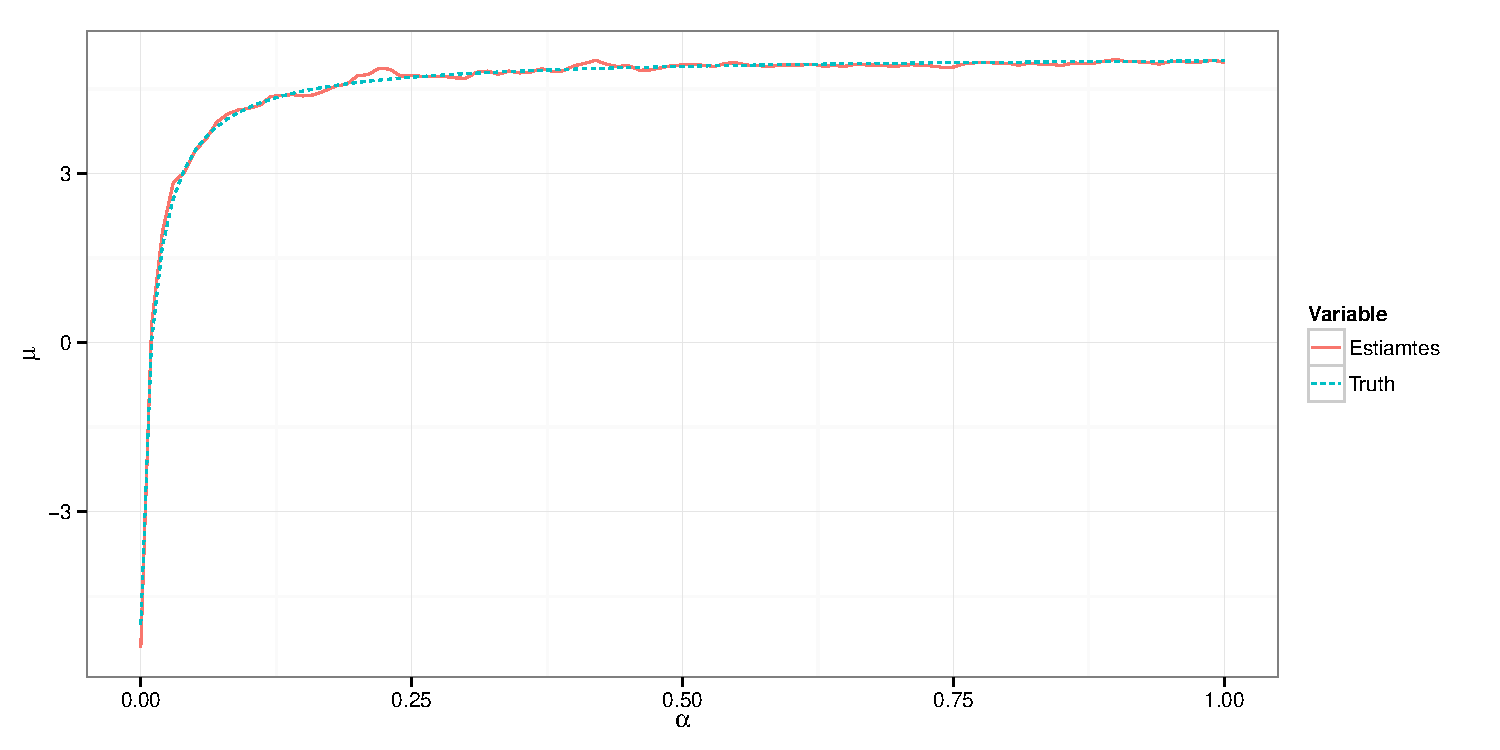
\includegraphics[width=\linewidth]{fig/mini_mu}
  \caption{The Monte Carlo estimates of the mean of the intermediate Normal
    distributions in the minimal example}
  \label{fig:mini mean}
\end{figure}

\begin{figure}
  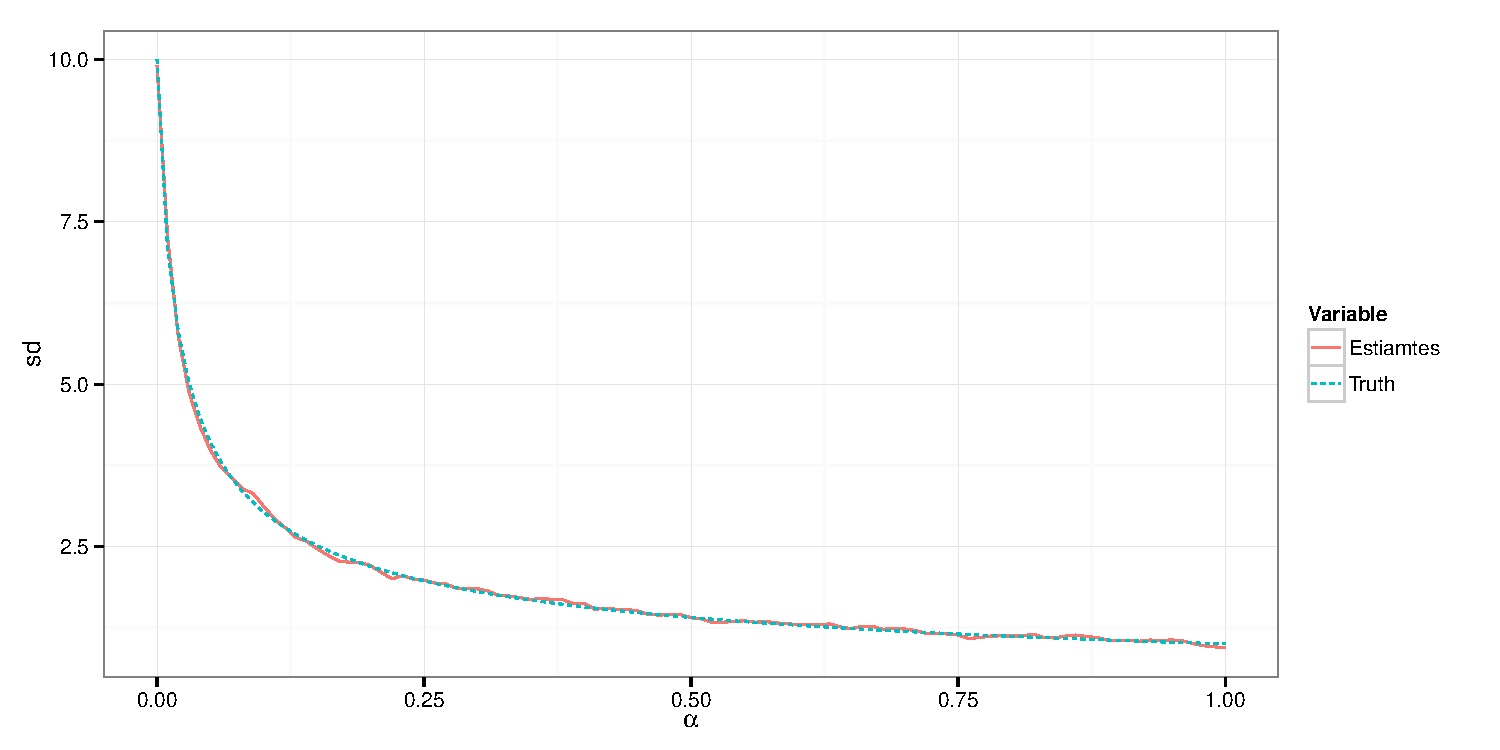
\includegraphics[width=\linewidth]{fig/mini_sd}
  \caption{The Monte Carlo estimates of the standard deviation of the
    intermediate Normal distributions in the minimal example}
  \label{fig:mini var}
\end{figure}

\section{Beyond the basics}
\label{sec:Beyond the basics}

The above example is quite minimal though it does show some advanced features
of the \vsmc library. In this section, we demonstrate the strength of the
presented framework by extend it with a few features. The first two shows that
it is trivial to implement the adaptive algorithms discussed in
section~\ref{sec:Extensions and refinements}. The third one shows that it is
easy to extend the framework with new algorithms, such as replacing the
built-in resampling algorithm.

\subsection{Implement the adaptive random walk scale}
\label{sub:Implement the adaptive random walk scale}

In the minimal example, we use the true standard deviation of the target
distribution for the Normal random walk. However, since we already implemented
a monitor that records the Monte Carlo estimates of the first and second raw
moments, it shall be trivial to use them to adaptively set the random walk
scales. To do this, we can use the \cppinline{pre_processor} member function
of the \cppinline{mini_move} class. Recall that, this member function is
called before any \cppinline{move_state} at each iteration. Here is the
modified \cppinline{mini_move} class,
\cppfile{code/mini_move_adaptive_scale.cpp}
The new class has a new member data \cppinline{sampler_}, which is a pointer
to the sampler. And through it, we can access the monitor named
\cppinline{"moments"}. The \cppinline{Monitor} class provides several ways to
read the record. Two of them are the overloaded \cppinline{record} member
function. It takes the index of the variable (starting with \cppinline{0}) as
its first argument. If no other arguments are provided, it simply returns the
most recent estimate. Alternatively, one can provide a second argument, which
shall be the iteration number. See the reference manual for details.

\subsection{Implement the CESS based adaptive schedule}
\label{sub:Implement the CESS based adaptive schedule}

To implement the \cess based adaptive schedule, again, we can use the member
function \cppinline{pre_processor} of the \cppinline{mini_move} class. In
\vsmc, the \cppinline{WeightSet} class provides the ability to compute the
value of $\cess/N$ (scaled to $[0,1]$) given (log) incremental weights. Below
is the modified \cppinline{mini_move} class,
\cppfile{code/mini_move_adaptive_schedule.cpp}
Now we have a member data \cppinline{alpha_}, which are simply indexed by the
iteration number. Inside member function \cppinline{pre_processor}, we make
sure that the first element is always $0$ and the last one is $1$. For any
value in between, we use a binary search to find the value that produce a new
target distribution with $\cess/N$ equal to a preset value $\cess^*/N$, which
we hard coded here as \cppinline{cess_star}. The call to
\cppinline{WeightSet::cess} takes an input iterator as its first argument, and
a boolean value, which indicate whether the incremental weights are on log
scale as its second argument. Now the \cppinline{alpha} member function no
longer compute $\alpha(t/T) = t/T$, instead it simply lookup in the vector
\cppinline{alpha_}.

\subsection{Use a new resampling algorithm}
\label{sub:Use a new resampling algorithm}

There are many areas of \vsmc algorithm been actively developed. Some of them
can be easy implemented with \vsmc through somehow ``creative'' use of the
classes like \cppinline{mini_move}, as demonstrated above. Other algorithms
may need to change \vsmc's internal. For example, \vsmc provide several
built-in resampling algorithms, which can be chosen through the constructor of
\cppinline{Sampler}. For example,
\begin{cppcode}
Sampler<mini> sampler(N, vsmc::Systematic);
\end{cppcode}
will construct a sampler with systematic resampling instead of the default
stratified resampling. Now consider that one has developed a new resampling
algorithm, to use it, one only need to define a function (or functor) similar
to the following,
\cppfile{code/resample.cpp}
where the input parameter \cppinline{N}, \cppinline{rng} and
\cppinline{weight} are the number of particles, an \cppoo{} \rng engine, and
the normalized weights, respectively. The output parameter
\cppinline{replication} shall be the number of replicates of each particle
after the resampling. To use it instead of one of the built-in algorithm, one
simply construct a sampler like the following,
\begin{cppcode}
Sampler<mini> sampler(N, resalg);
\end{cppcode}
Many advanced algorithms, including some recent development on parallel
resampling, are also possible though unavoidably, they will involve more
advanced \cpp techniques, which is beyond the scope of this chapter. See the
reference manual for details.

\section{Performance benchmark}
\label{sec:Performance benchmark}

One of the main motivation behind the creation of \vsmc is to ease the
parallelization with different programming models. The same implementation can
be used to built different samplers based on what kind of parallel programming
model is supported on the users' platforms. In this section we compare the
performance of various \smp parallel programming models and \opencl
parallelization. We use the Gaussian mixture model with \smc[2] algorithm as
shown in section~\ref{sub:Gaussian mixture model}. For a complete
documentation on its implementation with \vsmc, see \cite{vsmcjss}.

\subsection{Using the \protect\smp module}
\label{sub:Using the SMP module}

We consider five different implementations supported by \icpc~2013:
sequential, \tbb, \cilk, \openmp and \cppoo{} \cppinline{<thread>}. The
samplers are compiled with
\begin{makecode}
CXX=icpc -std=c++11 -gcc-name=gcc-4.7 -gxx-name=g++-4.7
CXXFLAGS=-O3 -xHost -fp-model precise  \
         -DVSMC_HAS_CXX11LIB_FUNCTIONAL=1  \
         -DVSMC_HAS_CXX11LIB_RANDOM=1
\end{makecode}
on a Ubuntu~12.10 workstation with an Xeon~W3550 (3.06GHz, 4 cores, 8 hardware
threads through hyper-threading) \cpu. A four components model and $100$
iterations with a prior annealing scheme is used for all implementations. A
range of numbers of particles are tested, from $2^3$ to $2^{17}$.

For different number of particles, the wall clock time and speedup are shown
in Figure~\ref{fig:bench-smp-perf}. For $10^4$ or more particles, the
differences are minimal among all the programming models. They all have
roughly 550\% speedup. With smaller number of particles, \vsmc's \cppoo
parallelization is less efficient than other industry strength programming
models. However, with $1000$ or more particles, which is less than typical
applications, the difference is not very significant.

\begin{figure}
  \centering
  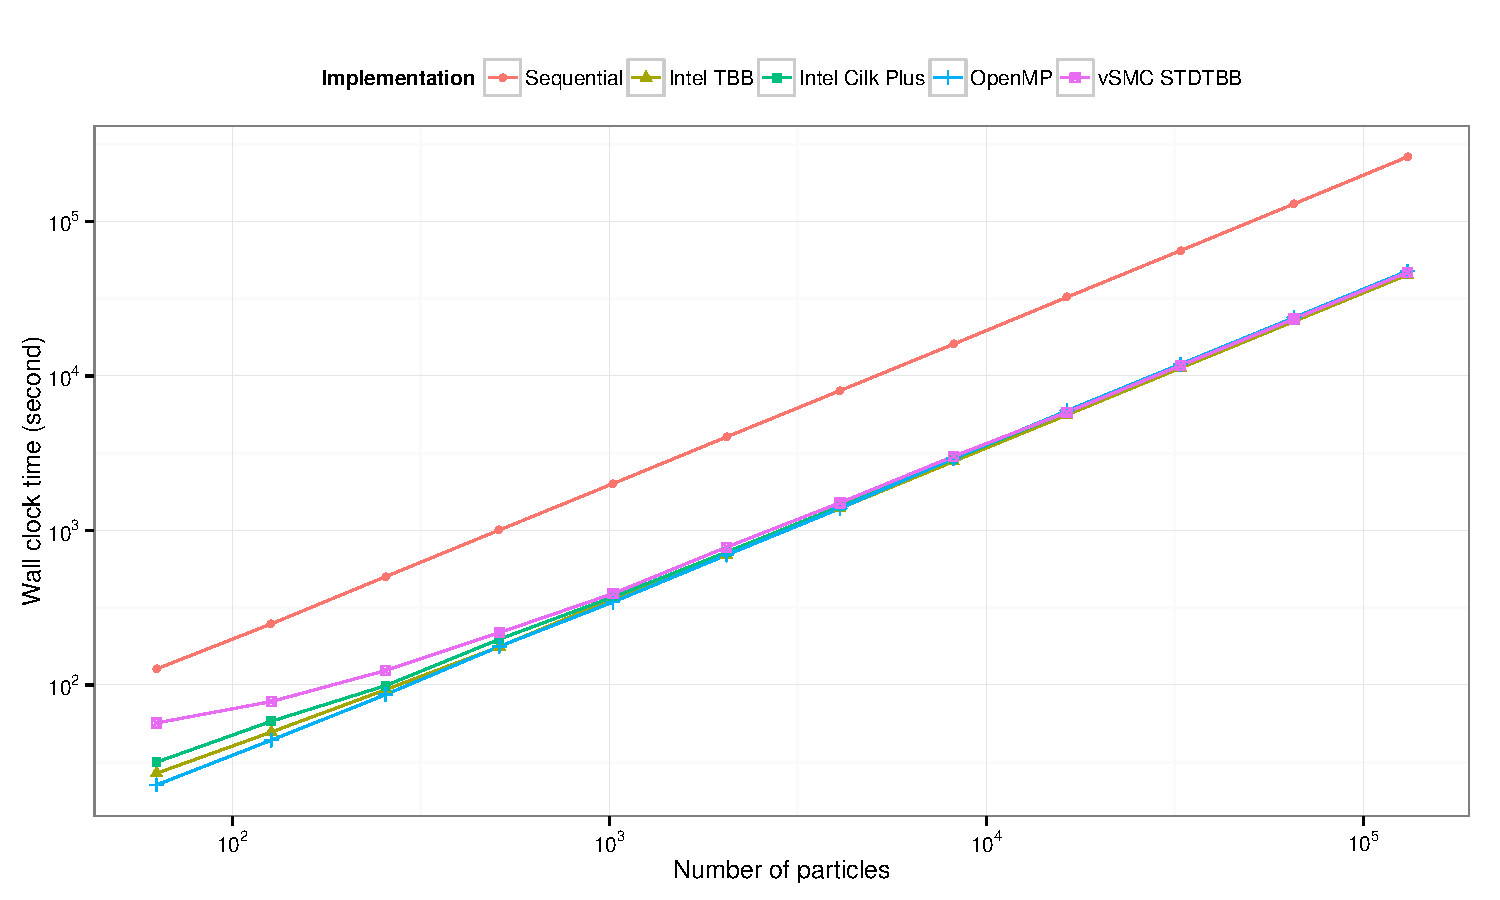
\includegraphics[width=\linewidth]{fig/bench-smp-time-running}
  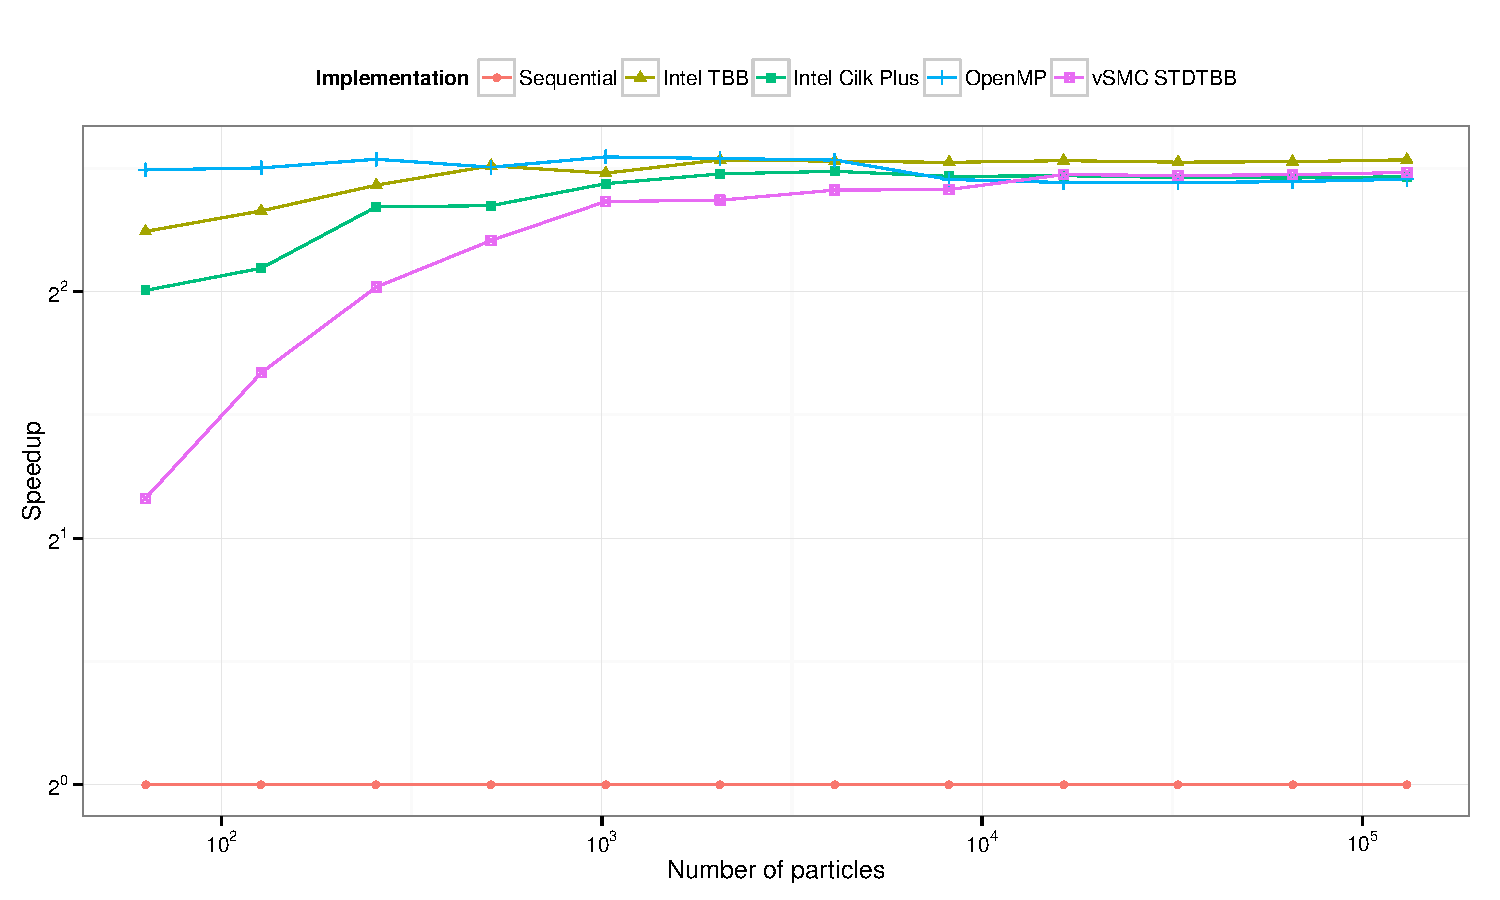
\includegraphics[width=\linewidth]{fig/bench-smp-speedup-running}
  \caption{Performance of \cpp implementations of Bayesian modeling for
    Gaussian mixture model (Linux; Xeon W3550, 3.06GHz, 4 cores, 8 threads).}
  \label{fig:bench-smp-perf}
\end{figure}

\subsection{Using the \protect\opencl module}
\label{sub:Using the OpenCL module}

The implementation of the same algorithm using \opencl is quite similar to
those using the \smp module.

\opencl implementations are also compared on the same workstation, which also
has an NVIDIA Quadro 2000 graphic card. \opencl programs can be compiled to
run on both \cpu and \gpu. For \cpu implementation, there are \iocl
\cite{iocl} and \aocl \cite{aocl} platforms. We use the \tbb implementation as
a baseline for comparison. The same \opencl implementation are used for all
the \cpu and \gpu runtimes.  Therefore they are not particularly optimized for
any of them. For the \gpu implementation, in addition to double precision, we
also tested a single precision configuration. Unlike modern \cpu, which have
the same performance for double and single precision floating point operations
(unless \simd instructions are used, which can have at most a speedup by a
factor of 2), \gpu penalize double precision performance heavily.

For different number of particles, the wall clock time and speed up are
plotted in Figure~\ref{fig:bench-ocl-perf}. With smaller number of particles,
the \opencl implementations have a high overhead when compared to the \tbb
implementation. With a large number of particles, \aocl has a similar
performance as the \tbb implementation. \iocl is about 40\% faster than the
\tbb implementation. This is due to more efficient vectorization and compiler
optimizations. The double precision performance of the NVIDIA \gpu has a 220\%
speedup and the single precision performance has near 1600\% speedup. As a
rough reference for the expected performance gain, the \cpu has a theoretical
peak performance of 24.48 GFLOPS. The \gpu has a theoretical peak performance
of 60 GFLOPS in double precision and 480 GFLOPS in single precision. This
represents 245\% and 1960\% speedup compared to the \cpu, respectively.

\begin{figure}
  \centering
  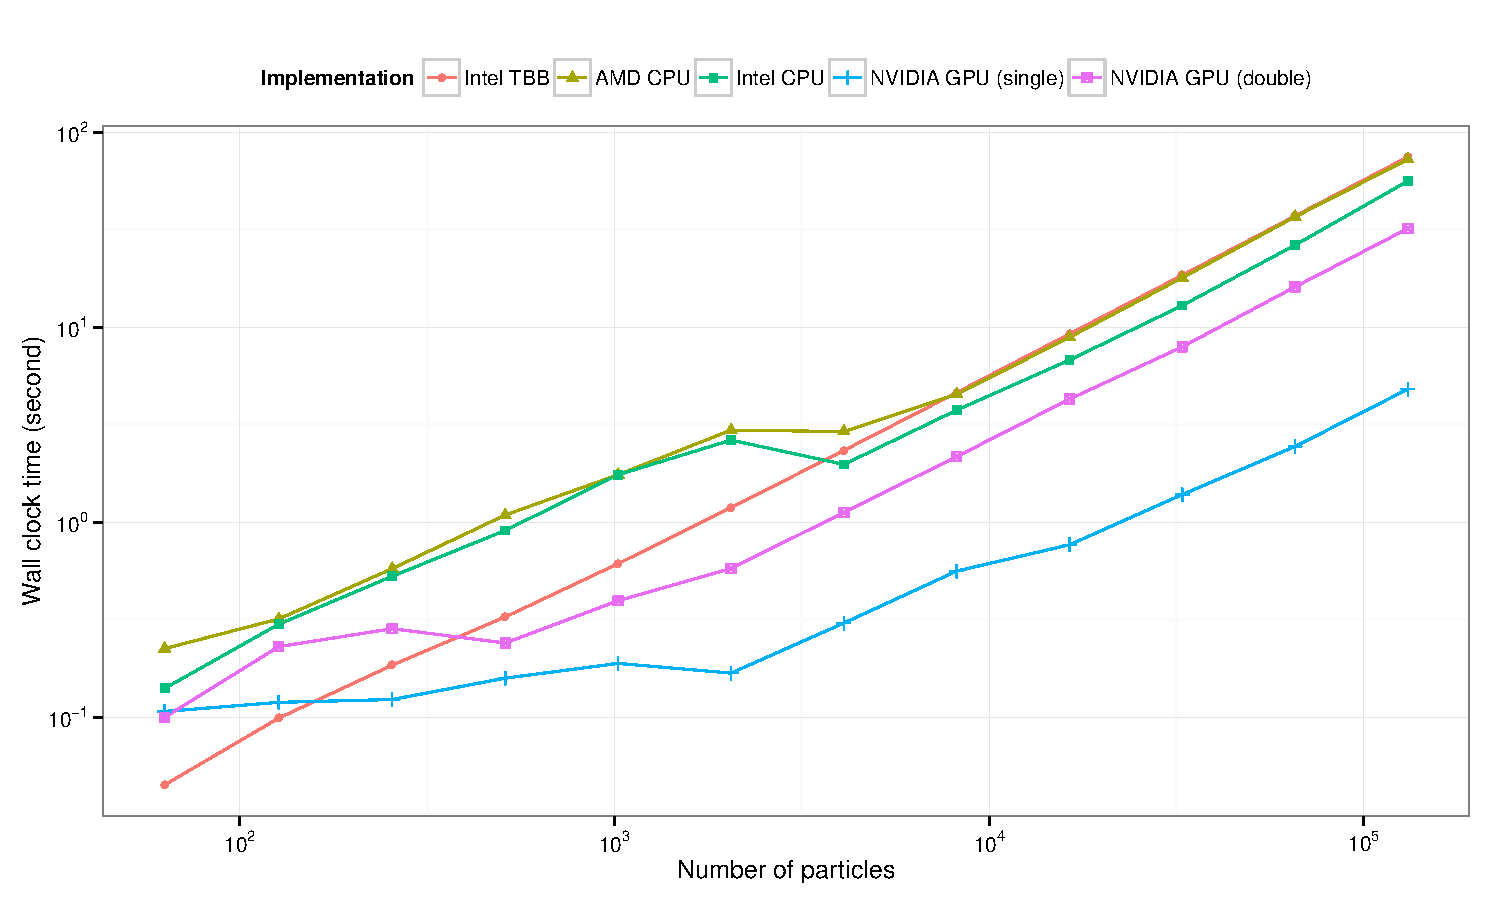
\includegraphics[width=\linewidth]{fig/bench-ocl-time-running}
  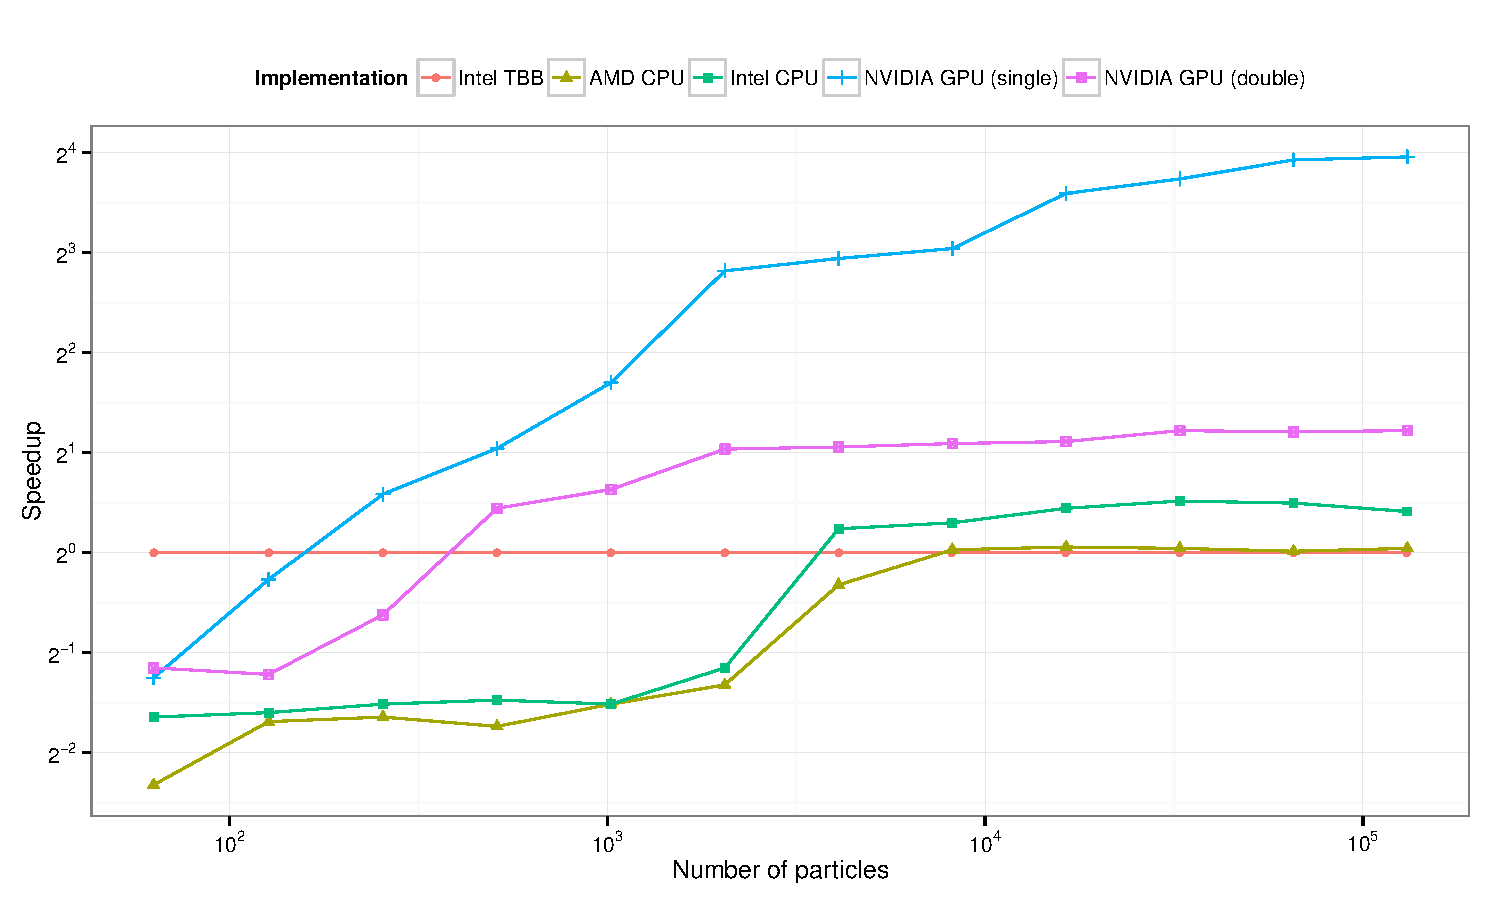
\includegraphics[width=\linewidth]{fig/bench-ocl-speedup-running}
  \caption{Performance of \opencl implementations of Bayesian modeling for
    Gaussian mixture model (Linux; Xeon W3550 \gpu, 3.06GHz, 4 cores, 8
    threads; NVIDIA Quadro 2000).}
  \label{fig:bench-ocl-perf}
\end{figure}

It is widely believed that \opencl programming is tedious and hard. However,
\vsmc provides facilities to manage \opencl platforms and devices as well as
common operations. Limited by the scope of this paper, the \opencl
implementation (distributed with the \vsmc source) is not documented in this
paper. Overall the \opencl implementation has about 800 lines including both
host and device code. It is not an enormous increase in effort when compared
to the 500 lines \smp implementation. Less than doubling the code base but
gaining more than 15 times performance speedup, we consider the programming
effort is relatively small.

\subsection{Core module}
\label{sub:Core module}

The core module abstracts general \smc samplers. \smc samplers can be viewed
as formed by a few concepts regardless of the specific problems. The following
is a list of the most commonly seen components of \smc samplers and their
corresponding \vsmc abstractions. Here and in the remaining of this chapter,
unless stated otherwise, all documented classes resides in the
\cppinline{vsmc} namespace.
\begin{itemize}
  \item A collection of all particle state values, namely
    $\{X_t^{(i)}\}_{i=1}^N$. In \vsmc, users need to define a class, say
    \cppinline{T}, to abstract this concept. We refer to this as the
    \emph{value collection}. We will slightly abuse the generic name
    \cppinline{T} in this chapter. Whenever a template parameter is mentioned
    with the name \cppinline{T}, it always refers to such a value collection
    type unless stated otherwise.
  \item A collection of all particle state values and their associated
    weights. This is abstracted by a \cppinline{Particle<T>} object. We refer
    to this as the \emph{particle collection}. A \cppinline{Particle<T>}
    object has three primary sub-objects. One is the above type \cppinline{T}
    value collection object. Another is an object that abstracts weights
    $\{W_t^{(i)}\}_{i=1}^N$. The last is a collection of \rng streams, one for
    each particle.
  \item Operations that perform tasks common to all samplers to these
    particles, such as resampling. These are the member functions of
    \cppinline{Particle<T>}.
  \item A sampler that updates the particles (state values and weights) using
    user defined callbacks. This is a \cppinline{Sampler<T>} object.
  \item Monitors that record the importance sampling estimates of certain
    functions defined for the values when the sampler iterates. These are
    \cppinline{Monitor<T>} objects. A monitor for the estimates of $E[h(X_t)]$
    computes $h(X_t^{(i)})$ for each $i = 1,\dots,N$. The function value
    $h(X_t)$ is allowed to be a vector.
\end{itemize}
Note that within the core module, all operations are applied to
\cppinline{Particle<T>} objects, that is $\{W_t^{(i)},X_t^{(i)}\}_{i=1}^N$,
instead of a single particle. Later we will see how to write operations that
can be applied to individual particles and can be parallelized easily.

\subsubsection{Program structures}
\label{ssub:Program structures}

A \vsmc program usually consists of the following tasks.
\begin{itemize}
  \item Define a value collection type \cppinline{T}.
  \item Constructing a \cppinline{Sampler<T>} object.
  \item Configure the behavior of initialization and updating by adding
    callable objects to the sampler object.
  \item Optionally add monitors.
  \item Initialize and iterate the sampler.
  \item Retrieve the outputs, estimates and other informations.
\end{itemize}
In this section we document how to implement each of these tasks. Within the
\vsmc library, all public classes, namespaces and free functions, are declared
in the namespace \cppinline{vsmc}.

\paragraph{A single particle}

If the value collection type \cppinline{T} satisfies certain
requirements\footnote{See the reference manual for technique details, it is
  sufficient to note here that \cppinline{StateMatrix} and any of its derived
  classes satisfy those requirements}, then for a \cppinline{Particle<T>}
object, one can construct a \cppinline{SingleParticle<T>} object that
abstracts one of the particle from the collection. For example,
\begin{cppcode}
Particle<T> particle(N);
SingleParticle<T> sp(i, &particle);
\end{cppcode}
create a \cppinline{SingleParticle<T>} object corresponding to the particle at
position \cppinline{i}. There are a few member functions of
\cppinline{SingleParticle<T>} that makes access to individual particles easier
than through the interface of \cppinline{Particle<T>}. We will demonstrate
some of them through examples in section~\ref{sec:Using the paralleization
  modules}.

\subsubsection{Initialization and updating}
\label{ssub:Initialization and updating}

All the callable objects that initialize, move and weight the particle
collection can be added to a sampler through a set of member functions. All
these objects operate on the \cppinline{Particle<T>} object. Because \vsmc
allows one to manipulate the particle collection as a whole, in principle many
kinds of parallelization are possible.

The initialization is set through \cppinline{Sampler}'s \cppinline{init}
member function,
\begin{cppcode}
Sampler<T> &init (const Sampler<T>::init_type &f)
\end{cppcode}
with a user defined callback. The callback type \cppinline{init_type} is a
type erasure (section~\ref{sub:Modern C++}), whose signature is as the
following,
\begin{cppcode}
std::size_t init_f (Particle<T> &, void *param);
\end{cppcode}
where \cppinline{param} can be used to pass arbitrary information used to
initialize the sampler.

The addition of updating methods is more flexible. There are two kinds of
updating methods. One is simply called \cppinline{move} in \vsmc, and is
performed before the possible resampling at each iteration. These moves
usually perform the updating of the weights among other tasks. The other is
called \cppinline{mcmc}, and is performed after the possible resampling. They
are often \mcmc type moves. Multiple \cppinline{move}'s or \cppinline{mcmc}'s
are also allowed. In fact a \vsmc sampler consists of a queue of
\cppinline{move}'s and a queue of \cppinline{mcmc}'s. The \cppinline{move}'s
in the queue can be changed through \cppinline{Sampler<T>::move},
\begin{cppcode}
Sampler<T> &move (const Sampler<T>::move_type &f, bool append);
\end{cppcode}
The type erasure \cppinline{move_type} has the signature,
\begin{cppcode}
std::size_t move_f (std::size_t iter, Particle<T> &);
\end{cppcode}
where the \cppinline{iter} is the iteration number with the initialization
step count as $0$. If \cppinline{append == true} then \cppinline{f} is
appended to the existing (possibly empty) queue. Otherwise, the existing queue
is cleared and \cppinline{f} is added.

\subsubsection{Running the algorithm, monitoring and outputs}
\label{ssub:Running the algorithm, monitoring and outputs}

Having set all the operations, one can initialize and iterate the sampler by
calling
\begin{cppcode}
sampler.initialize((void *)param);
sampler.iterate(iter_num);
\end{cppcode}
The \cppinline{param} argument to \cppinline{initialize} is optional, with
\cppinline{NULL} as its default. This parameter is passed to the user defined
callback. The \cppinline{iter_num} argument to \cppinline{iterate} is also
optional; the default is $1$.

Before initializing the sampler or after a certain time point, one can add
monitors to the sampler. The concept is similar to \bugs's \cppinline{monitor}
statement, except it does not monitor the individual values but rather the
importance sampling estimates. Consider approximating $\Exp[h(X_t)]$, where
$h(X_t) = (h_1(X_t),\dots,h_m(X_t))$ is an $m$-vector function. The importance
sampling estimate can be obtained by $AW$ where $A$ is an $N$ by $m$ matrix
where $A(i,j) = h_j(X_t^{(i)})$ and $W = (W_t^{(i)},\dots,W_t^{(N)})^T$ is the
$N$-vector of normalized weights. To compute this importance sampling
estimate, one need to define the following evaluation function (or other kinds
of callable objects),
\cppfile{code/monitor_eval.cpp}
and add it to the sampler by calling,
\begin{cppcode}
sampler.monitor("variable.name", m, monitor_eval);
\end{cppcode}
When the function \cppinline{monitor_eval} is called, \cppinline{iter} is the
iteration number of the sampler, \cppinline{m} is the same value as the one
the user passed to \cppinline{Sampler<T>::monitor}; and thus one does not need
global variable or other similar techniques to access this value. The output
pointer \cppinline{res} points to an $N \times m$ output array of row major
order. That is, after the calling of the function,
\cppinline{res[i * dim + j]} shall be $h_j(X_t^{(i)})$.

After each iteration of the sampler, the importance sampling estimate will be
computed automatically. See the reference manual for various ways to retrieve
the results. Usually it is sufficient to output the sampler by
\begin{cppcode}
std::ofstream output("file.name");
output << sampler << std::endl;
\end{cppcode}
where the output file will contain the importance sampling estimates among
other things. Alternatively, one can use the \cppinline{Monitor<T>::record}
member function to access specific historical results. See the reference
manual for details of various overloaded version of this member function.

\subsubsection{Implementing initialization and updating}
\label{ssub:Implementing initialization and updating}

So far we have only discussed how to add initialization and updating objects
to a sampler. To actually implement them, one writes callable objects that
operate on the \cppinline{Particle<T>} object. For example, a move can be
implemented through the following function as mentioned before,
\begin{cppcode}
std::size_t move_f (std::size_t iter, Particle<T> &particle);
\end{cppcode}
Inside the body of this function, one can change the value by manipulating the
object through the reference returned by \cppinline{particle.value()}.

The weights can be updated through a set of member functions of
\cppinline{WeightSet}. For example,
\begin{cppcode}
std::vector<double> weight(particle.size());
particle.weight_set().set_equal_weight();
particle.weight_set().set_weight(weight.begin());
particle.weight_set().mul_weight(weight.begin());
particle.weight_set().set_log_weight(weight.begin());
particle.weight_set().add_log_weight(weight.begin());
\end{cppcode}
The \cppinline{set_equal_weight} member function sets all weights to be equal.
Similarly, the \cppinline{set_weight} and \cppinline{set_log_weight} member
functions set the values of weights and logarithm weights, respectively. And
the \cppinline{mul_weight} and \cppinline{add_log_weight} member functions
multiply the weights or add to the logarithm weights by the given values,
respectively. All these member functions accept general input iterators as
their arguments.

One important thing to note is that, whenever one of these member functions is
called, both the weights and logarithm weights will be re-calculated,
normalized, and the \ess will be updated. The reason for not allowing changing
a single particle's weight is that, in a multi-threading environment, it is
possible for one to change one weight in one thread, and obtain another in
another thread without proper normalizing. Conceptually, changing one weight
actually changes all weights.

\subsubsection{Generating random numbers}
\label{ssub:Generating random numbers}

The \cppinline{Particle<T>} object has a sub-object, a collection of \rng
engines that can be used with \cppoo{} \cppinline{<random>} or \boost
distributions. For each particle \cppinline{i}, one can obtain an engine that
produces an \rng stream independent of others by
\begin{cppcode}
particle.rng(i);
\end{cppcode}
To generate distribution random variates, one can use the
\cppoo{} \cppinline{<random>} library. For example,
\begin{cppcode}
std::normal_distribution<double> rnorm(mean, sd);
double r = rnorm(particle.rng(i));
\end{cppcode}
or use the \boost library,
\begin{cppcode}
boost::random::normal_distribution<double> rnorm(mean, sd);
double r = rnorm(particle.rng(i));
\end{cppcode}
\vsmc itself also makes use of \cppoo{} \cppinline{<random>} or \boost
depending on the value of the configuration macro
\cppinline{VSMC_HAS_CXX11LIB_RANDOM}. Though the user is free to choose which
one to use in their own code, there is a convenient alternative. For each
class defined in \cppoo{} \cppinline{<random>}, it is imported to the
\cppinline{vsmc::cxx11} namespace. Therefore one can use
\begin{cppcode}
cxx11::normal_distribution<double> rnorm(mean, sd);
\end{cppcode}
while the underlying implementation of \cppinline{normal_distribution} can be
either \cppoo standard library or \boost. The benefit is that if one needs to
develop on multiple platforms, and only some of them support \cppoo and some
of them have the \boost library, then only the configure macro
\cppinline{VSMC_HAS_CXX11LIB_RANDOM} needs to be changed. This can be
configured through \cmake and other build systems. Of course, one can also use
an entirely different \rng system than those provided by \vsmc.

\subsection{SMP module}
\label{sub:SMP module}

\subsubsection{Sequential and parallel implementations}
\label{ssub:Sequential and parallel implementations}

In the last section we introduce the \cppinline{SingleParticle<T>} concept.
Though it, we can write implementations of \smc algorithms that manipulate a
single particle and can be applied to all particles in parallel or
sequentially. For sequential implementations, this can be done through five
base classes,
\begin{cppcode}
template <typename BaseState> class StateSEQ;
template <typename T, typename D = Virtual> class InitializeSEQ;
template <typename T, typename D = Virtual> class MoveSEQ;
template <typename T, typename D = Virtual> class MonitorEvalSEQ;
template <typename T, typename D = Virtual> class PathEvalSEQ;
\end{cppcode}
As usual with templates, the type \cppinline{BaseState} and \cppinline{T} need
to satisfy certain requirements. It is sufficient to note here that the
\cppinline{StateMatrix} class introduced earlier can be used. The details of
all these class templates can be found in the reference manual.  Here we use
the \cppinline{MoveSEQ<T>} class as an example to illustrate their usage.
Recall that \cppinline{Sampler<T>} expect a callable object which has the
following signature as a move,
\begin{cppcode}
std::size_t move_f (std::size_t iter, Particle<T> &particle);
\end{cppcode}
For the purpose of illustration, the type \cppinline{T} is defined as,
\begin{cppcode}
typedef StateMatrix<RowMajor, 1, double> T;
\end{cppcode}
Here is a typical example of implementation of such a function,
\cppfile{code/move_f.cpp}
where \cppinline{cal_inc_weight} is some function that calculates the
logarithm incremental weights. As we see, there are three main parts of a
typical move. First, we allocate a vector \cppinline{inc_weight}. Second, we
generate normal random variates for each particle and calculate the
incremental weights. This is done through a \cppinline{for} loop. Third, we
add the logarithm incremental weights. The first and the third are
\emph{global} operations while the second is \emph{local}. The first and the
third are often optional and absent. The local operation is also usually the
most computational intensive part of \smc algorithms and can benefit the most
from parallelizations.

With \cppinline{MoveSEQ<T>}, which defines the \cppinline{operator()} as
required by the core module interface,
\begin{cppcode}
std::size_t operator() (std::size_t iter, Particle<T> &particle);
\end{cppcode}
one can derive from this class, and customize what this operator does by
defining one or more of the following three member functions, corresponding to
the three parts, respectively,
\begin{cppcode}
void pre_processor (std::size_t iter, Particle<T> &particle);
std::size_t move_state (std::size_t iter, SingleParticle<T> sp);
void post_processor (std::size_t iter, Particle<T> &particle);
\end{cppcode}
For example,
\cppfile{code/move_class.cpp}
The \cppinline{operator()} of \cppinline{MoveSEQ<T>} is equivalent to the
single function implementation as shown before.

In the simplest case, \cppinline{MoveSEQ} only takes away the loop around
Part~2. However if one implement the move in such a way, and then replace
\cppinline{MoveSEQ} with \cppinline{MoveOMP}, the changing of the base class
name causes \vsmc to use \openmp to parallelize the loop. For example, one can
declare the class as
\begin{cppcode}
#include <vsmc/smp/backend_omp.hpp>
class move : public MoveOMP<T>;
\end{cppcode}
and use exactly the same implementation as before. Now when the member
function \cppinline{move::operator()} is called, it will be parallelized by
\openmp. Other backends are available in case \openmp is not available. Among
them there are \cilk and \tbb. In addition to these well known parallelization
programming models, \vsmc also has its own implementation using \cppoo{}
\cppinline{<thread>}. There are other backends documented in the reference
manual. To use any of these parallelization, all one need to do is to change a
few base class names. In practice, one can use conditional compilation, for
example, to use a sequential implementation or a \openmp parallelized one, we
can write,
\begin{cppcode}
#ifdef USE_SEQ
#include <vsmc/smp/backend_seq.hpp>
#define BASE_MOVE MoveSEQ
#endif

#ifdef USE_OMP
#include <vsmc/smp/backend_omp.hpp>
#define BASE_MOVE MoveOMP
#endif

class move : public BASE_MOVE<T>;
\end{cppcode}
And we can compile the same source into different samplers with
\shinline{Makefile} rules such as the following,
\begin{makecode}
prog-seq : prog.cpp
        $(CXX) $(CXXFLAGS) -DUSE_SEQ -o prog-seq prog.cpp
prog-omp : prog.cpp
        $(CXX) $(CXXFLAGS) -DUSE_omp -o prog-omp prog.cpp
\end{makecode}
Or one can configure the source file through a build system such as \cmake,
which can also determine which programming model is available on the system.

\subsubsection{Adapter}
\label{ssub:Adapter}

Sometimes, the cumbersome task of writing a class to implement a move and
other operations can out weight the power we gain through object oriented
programming. For example, a simple \cppinline{move_state}-like function is all
that we need to get the work done. In this case, one can create a move through
the \cppinline{MoveAdapter}. For example, say we have implemented
\begin{cppcode}
std::size_t move_state (std::size_t iter, SingleParticle<T> sp);
\end{cppcode}
as a function. Then one can create a callable object through
\begin{cppcode}
MoveAdapter<T, MoveSEQ>  move_obj(move_state);
MoveAdapter<T, MoveSTD>  move_obj(move_state);
MoveAdapter<T, MoveTBB>  move_obj(move_state);
MoveAdapter<T, MoveCILK> move_obj(move_state);
MoveAdapter<T, MoveOMP>  move_obj(move_state);
sampler.move(move_obj, false);
\end{cppcode}
These are respectively, sequential, \cppoo{} \cppinline{<thread>}, \tbb,
\cilk, and \openmp implementations. The first template parameter is the type
of value collection and the second is the name of the base class template.
Actually, the \cppinline{MoveAdapter}'s constructor accepts two optional
arguments, the \cppinline{pre_processor} and the \cppinline{post_processor},
corresponding to the other two aforementioned member functions. Similar
adapters for the other three base classes also exist.

Another scenario where an adapter is desired is that which backend to use
needs be decided at runtime. The above simple adapters can already be used for
this purpose. In addition, another form of the adapter is as the following,
\begin{cppcode}
class move;
MoveAdapter<T, MoveTBB, move> move_obj;
sampler.move(move_obj, false);
\end{cppcode}
where the class \cppinline{move} has the same definition as before but it no
longer derives from any base class. The class \cppinline{move} is required to
have a default constructor, a copy constructor and an assignment operator.

\subsection{Thread-safety and scalability considerations}
\label{sub:Thread-safety and scalability considerations}

When implementing parallelized \smc algorithms, issues such as thread-safety
cannot be avoided even though the \vsmc library hides most parallel constructs
from the user.

Classes in the \vsmc library usually guarantee that their member functions are
thread-safe in the sense that calling the same member function on different
objects at the same time from different threads is safe. However, calling
mutable member functions on the same object from different threads is usually
not safe. Calling immutable member functions is generally safe. There are a
few exceptions,
\begin{itemize}
  \item The constructors of \cppinline{Particle} and \cppinline{Sampler} are
    not thread-safe. Therefore if one need to construct multiple
    \cppinline{Sampler} from different threads, a mutex protection is needed.
    However, subsequent member function calls on the constructed objects are
    thread-safe according to the above rules.
  \item Member functions that concern a single particle are generally
    thread-safe in the sense that one can call them on the same object from
    different threads as long as they are called for different particles. For
    example \cppinline{Particle::rng} and \cppinline{StateMatrix::state} are
    thread-safe.
\end{itemize}
In general, one can safely manipulate different individual particles from
different threads, which is the minimal requirement for scalable
parallelization. But one cannot manipulate the whole particle collection from
different threads, for example \cppinline{WeightSet::set_log_weight}.

User defined callbacks shall generally follow the same rules. For example, for
a \cppinline{MoveOMP} subclass, \cppinline{pre_processor} and
\cppinline{post_processor} does not have be thread-safe, but
\cppinline{move_state} needs to be. In general, avoid write access to memory
locations shared by all particles from \cppinline{move_state} and other
similar member functions. One needs to take some extra care when using
third-party libraries. For example, in our example implementation of the
\cppinline{move} class, the \cppinline{rnorm} object, which is used to
generate Normal random variates, is defined within \cppinline{move_state}
instead of being a class member data even though it is created with the same
parameters for each particle. This is because the call
\cppinline{rnorm(sp.rng())} is not thread-safe in some implementations, for
example, when using the \boost library.

For scalable performance, certain practices should be avoided when
implementing member functions such as \cppinline{move_state}. For example,
dynamic memory allocation is usually lock-based and thus should be avoided.
Alternatively one can use a scalable memory allocator such as the one provided
by \tbb. In general, in functions such as \cppinline{move_state}, one should
avoid using locks to guarantee thread-safety, which can be a bottleneck to
parallel performance.
